\section{Vidas}
O conceito do jogo é simples, existem chaves, existe um local final, existem torres e existem balas. Como tal optamos por colocar "vidas", digamos que o jogador começa com um determinado numero de vidas, perdendo uma por cada vez que é atingido por uma bala.

\begin{figure}[here]
                 \centering{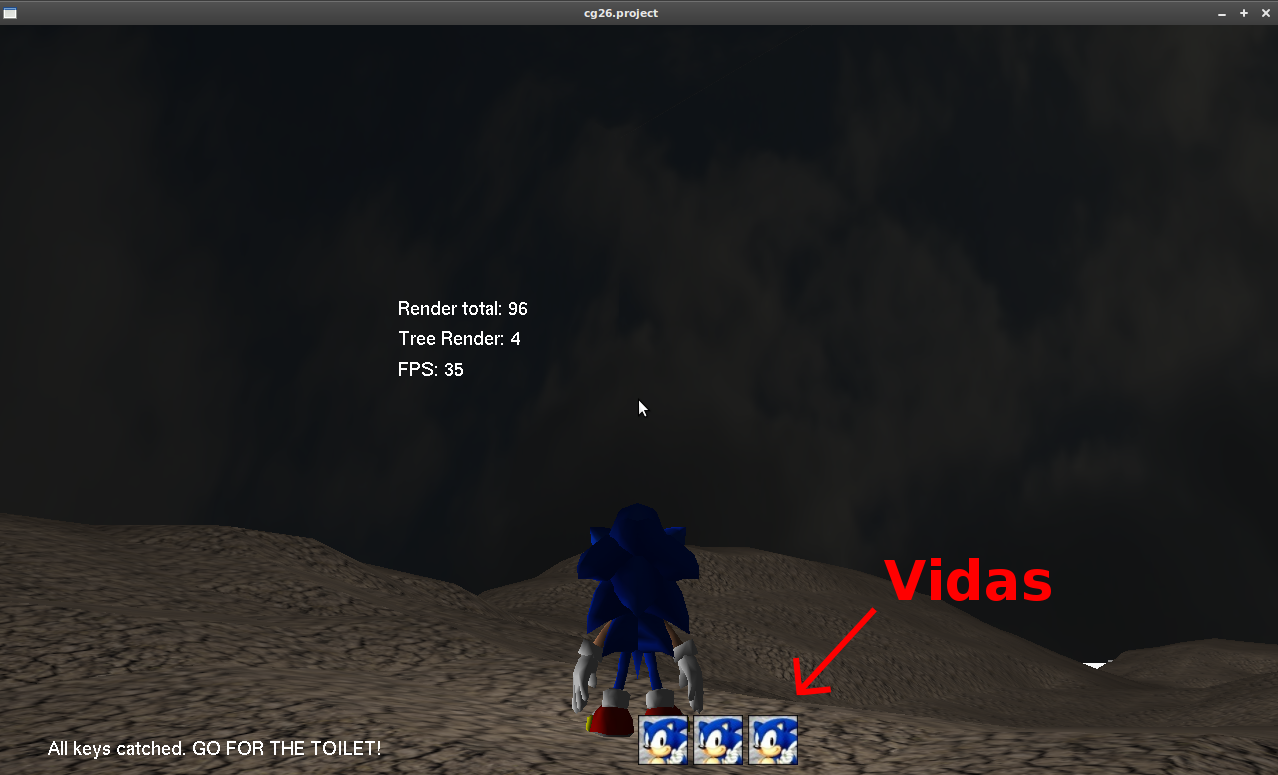
\includegraphics[width=0.8\textwidth]{images/lifes.png}}
                 \caption{Screenshot para as vidas.}
                 \label{fig:prototype}
\end{figure}